% Five books on three shelves. Counts 2, 2, 1. Some shelf has at least ceil(5/3)=2.
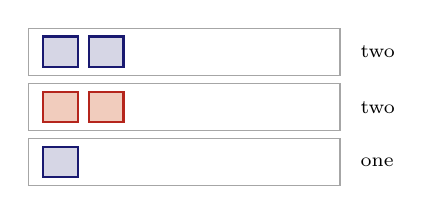
\begin{tikzpicture}[x=0.55cm,y=0.7cm]
  \foreach \shelf in {0,1,2} {
    \draw[gray!70] (0,\shelf) rectangle (7.2,\shelf+0.85);
  }
  % shelf 2 (top): two books
  \draw[MidnightBlue,thick,fill=MidnightBlue!18] (0.35,2.15) rectangle (1.15,2.7);
  \draw[MidnightBlue,thick,fill=MidnightBlue!18] (1.4,2.15) rectangle (2.2,2.7);
  % shelf 1: two books
  \draw[BrickRed,thick,fill=BrickRed!18] (0.35,1.15) rectangle (1.15,1.7);
  \draw[BrickRed,thick,fill=BrickRed!18] (1.4,1.15) rectangle (2.2,1.7);
  % shelf 0: one book
  \draw[MidnightBlue,thick,fill=MidnightBlue!18] (0.35,0.15) rectangle (1.15,0.7);
  \node[font=\scriptsize,anchor=west] at (7.45,2.42) {two};
  \node[font=\scriptsize,anchor=west] at (7.45,1.42) {two};
  \node[font=\scriptsize,anchor=west] at (7.45,0.42) {one};
\end{tikzpicture}
